\documentclass[letterpaper]{article}
\usepackage{underscore}
\usepackage[left=2.0cm, right=2.0cm, top=2.0cm]{geometry}
\usepackage[utf8]{inputenc}
\usepackage{graphicx}
\usepackage{graphics}
\usepackage[spanish]{babel}
\usepackage{lipsum}
\usepackage{float}
\usepackage{subfigure}

\title{EV\_1\_6\_Explicar\_la\_operación\_de\_los\_circuitos\_de\_activación\_con\_tristores\_en\_convertidores\_CA-CD\_y\_CA-CA}
\author{Alcantar Diaz Joel Alejandro.}
\date{24/09/2019}

\begin{document}

    \maketitle
    \begin{center}
        
\includegraphics[scale=0.5]{IMG/UPZMGlog.png}\\
        \vspace{2cm}
    \textbf{Univercidad Politécnica de la Zona Metropolitana de Guadalajara $|$ Ing. Mecatrónica 4$^{to}$ $"$A$"$}
    \end{center}
    \newpage
    \begin{large}
        \textbf{¿Que es un tiristor?}\\\\
        Un tiristor es un componente que funciona de manera similar a un relevador pero con diferencias muy marcadas, algunas de ellas son:
        \begin{enumerate}
            \item No tienen componentes mecanicos.
            \item Solo conducen la corriente en un sentido.
            \item Pueden conducir corrieentes muy altas.
            \item Pueden soportar tensiones muy altas.
            \item Tienen mucha mas vida util.
            \newline
        \end{enumerate}
        Su apariencia es la un encapsulado comun para transistores y la mas comun es la TO-220.
        \begin{figure}[htbp]
            \centering
            \subfigure[Delantero]{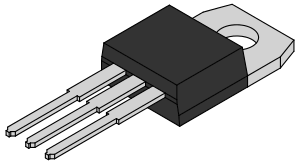
\includegraphics[scale=0.7]{IMG/to220f.png}}
            \subfigure[Trasero]{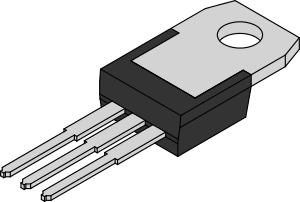
\includegraphics[scale=0.7]{IMG/to220b.png}}
            \caption{Encapsulado TO-220}
            \label{fig:my_label}
        \end{figure}\\
        \begin{large}
            \textbf{Tiristores en convertidores CA-CD}\\\\
            Los tiristores en este tipo de convertidor se pueden usar como reguladores de voltaje seleccionando la parte de la onda que se desea obtener, entre mayor sea el desface menor sera el voltaje hasta que se llegue a 90º. A partir de 90º el voltaje de la onda se vuelve inverso y su corriente es 0, en este caso se requiere que la carga en el circuito genere una corriente.\\
            Por ejemplo, si se conecta una bateria mientras el tiristor captura una parte de la onda menor a 90º esta estara cargando, pero si el angulo de desface supera los 90º la bateria comenzara a descargarce por que el circuito toma la corriente de la bateria.\\\\
            Para calcular el voltaje medio de salida se utiliza la formula:\\\\
                \begin{figure}[htbp]
                    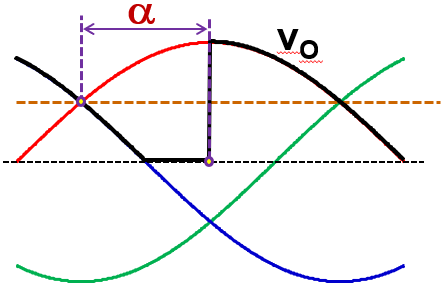
\includegraphics[scale=0.5]{IMG/ond1.png}
                    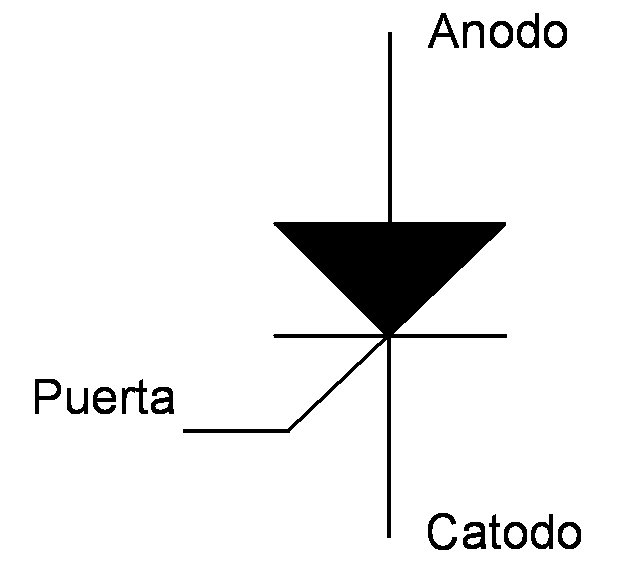
\includegraphics[scale=0.3]{IMG/tiri.jpg}
                    \label{fig:my_lab55el}
                \end{figure}\newpage
                \textbf{$\frac{3}{2\pi}\int ^{\pi}_{\frac{\pi}{6}+\alpha}V_g \cdot sen(\omega_{red}\cdot t)=\frac{3}{2\pi}V_g \cdot(1+sen(\frac{\pi}{3}-\alpha))$}\\\\
            \textbf{Tiristores en convertidores CA-CA}\\\\
            Tambien llamados controladores de face se comportan de manera similar a solo que estos son mas bien reductores de potencia que son muy empleados para regular luces por ejemplo, la velocidad de un motor, entre otras funciones.\\
            Uno de los circuitos mas simpples es con una resistencia que regula el tiempo de carga de un capacitor que activa un diac y ese diac ativa al triac que deja pasar la corriente por el circuito primario.
        \end{large}
    \end{large}
    \bibliographystyle{plain}
    \bibliography{Bib.bib}
\end{document}
